\documentclass[twocolumn,twoside]{svmultivs_gm} %please do not change this line
\usepackage{graphicx}
\usepackage{siunitx}
% \usepackage{subcaption}
\usepackage{multicol}
\usepackage{colortbl}
\usepackage{multirow}
\usepackage{tabularx}
\usepackage{makecell}
\usepackage{url}

\title*{NMA Analysis Center -- Progress Report}
% \subtitle{Optional Sub-title on first page}
\titlerunning{Progress Report}
%  The contents of \title* are printed on the first page.
% The contents of \subtitle are printed below the title on the first page.  This keyword is optional.
% The contents of \titlerunning are printed on the other pages.
% This should be a short version of the title.
%  Example:
% \title*{Investigation into Radio Frequency Interfence at VLBI Stations} \subtitle{A Study of Five Cases}
% \titlerunning{RFI Investigation}
\author{Ann-Silje Kirkvik, Geir Arne Hjelle, {\AA}smund Skj{\ae}veland, Michael D\"ahnn, Ingrid Fausk}
\authorrunning{Kirkvik et al.} %see comments below
\authoremails{ann-silje.kirkvik@kartverket.no geir.arne.hjelle@kartverket.no asmund.skjaeveland@kartverket.no}
\institute{Norwegian Mapping Authority}
%  \author and \institute keywords:
%  Each number in \author refers to an institution with which the author is associated.
% The numbers should correspond to numbered institutions in the \institute keyword.
% If all authors are associated with only one institution (the same institution), then the numbers should be omitted
% from \author and \institute.
% If an author is associated with two or more institutions, multiple numbers may be used.
%  The \institute key word must be a single line.
% Please separate institutions using \\ between each institution.
%  \authorrunning keyword:
%  For one author, please use \authorrunning{last_name_of_author}, e.g., \authorrunning{Gordon} For two authors, please
% use \authorrunning{last_name_of_first_author and last_name_of_second_author} e.g., \authorrunning{Gordon and
% MacMillan} For three or more authors, please use \authorrunning{last_name_of_first_author et al.} e.g.,
% \authorrunning{Gordon et al.}  Examples:
%  \author{Dirk Behrend} \authorrunning{Behrend} \author_emails{dirk.behrend-1@nasa.gov} \institute{NVI, Inc.} 
% \author{Karen Baver, Dirk Behrend} \authorrunning{Baver and Behrend}
% \author_emails{karen.d.baver@nasa.gov,dirk.behrend-1@nasa.gov} \institute{NVI, Inc.}  \author{John Gipson~$^1$, David
% Eriksson~$^{1,2}$, Dan MacMillan~$^1$} \authorrunning{Gipson et al.| \institute{1. NVI, Inc.\\ 2. Chalmers University
% of Technology}
\ContactAuthorName{Ann-Silje Kirkvik}
\ContactAuthorTelephone{+4732118421}
\ContactAuthorEmail{ann-silje.kirkvik@kartverket.no}
%  \ContactAuthorName, \ContactAuthorTelephone, and \ContactAuthorEmail should be used to identify the preferred contact
% author.
\NumberofInstitutions{1}
\InstitutionPostAddress{1}{Postboks 600 Sentrum, 3507 H{\o}nefoss}
\InstitutionCountry{1}{Norway}
\InstitutionWebPage{1}{www.kartverket.no}
% \InstitutionPostAddress{2}{N.A} \InstitutionCountry{2}{N.A} \InstitutionWebPage{2}{N.A}  Please change
% \NumberofInstitutions as needed.
% Please add or delete \InstitutionPostAddress, \InstitutionCountry, and \InstitutionWebPage as needed.
%  The keywords \InstitutionPostAddress, \InstiutionCountry, and \InstitutionWebPage are required to let the IVS
% publications software operate.  But the contents of these keywords may be any value for the IVS General Meeting
% Proceedings. So the content may be kept as N.A.
% or filled in.
\begin{document}  %please do not change this line
\maketitle       %please do not change this line
\abstract{The Norwegian Mapping Authority is currently developing \textbf{Where}, a new software for geodetic
analysis.
The software will be used to analyze VLBI sessions and contribute to the rapid and other operational products of the International VLBI Service for Geodesy and
Astrometry (IVS). All the components needed for a single session VLBI analysis in Where are finished and the software is in its final
testing phase. Together with the IVS Combination Center the quality of the processed solutions are being evaluated and improved as
problems are detected. The goal is to have a fully working version of the VLBI part of the software before the end of 2018.}
\keywords{VLBI, Where, Software, Analysis}
%  Please fill in one or more keywords in \keywords{}.
% One to five keywords is the suggested range.
\section{Introduction}
The Norwegian Mapping Authority (NMA) has been an Associate Analysis Center within the IVS (\cite{behrend2013},
\cite{schuh2012}) since 2010.  The original plan was to use the GEOSAT software~\cite{kierulf2010} and become an
operational analysis center which regularly processes R1 and R4 sessions. As previously reported in the IVS 2015+2016
Biennial Report~\cite{kirkvik2017a}, the GEOSAT software was abandoned and a new software is under development. The new
software is called \textbf{Where} \cite{kirkvik2017b}. NMA plans to use this software
to submit timely analyses to the IVS Combination Center (CCIVS).

\section{Motivation}

NMA has operated the VLBI station in Ny-{\AA}lesund since the beginning of the 1990s with the first observations in
1994. The site is currently being upgraded with two new VLBI stations and a SLR station is planned added to the site by
2022. Several GNSS stations and a DORIS beacon already exist in Ny-{\AA}lesund.

Ny-{\AA}lesund is situated at \ang{78,55}N, \ang{11,56}E on the west coast of Spitsbergen, the largest island in the
Svalbard archipelago. Ny-{\AA}lesund is not open to the general public and professionals working there are limited to
fixed term contracts. This naturally causes a high turnover and finding qualified personnel for a small field of
science, such as VLBI and SLR, is a continuous challenge. Having qualified personnel in permanent positions at the head
office is therefore essential. Creating, maintaining and using an analysis software provides valuable compentence and
insights into the field of VLBI for the group at the head office. Additionally -- by becoming an analysis center NMA can finally analyze the
data collected at Ny-{\AA}lesund and provide direct feedback to the station on its performance.

\section{Software}


\begin{figure}[!htbp]
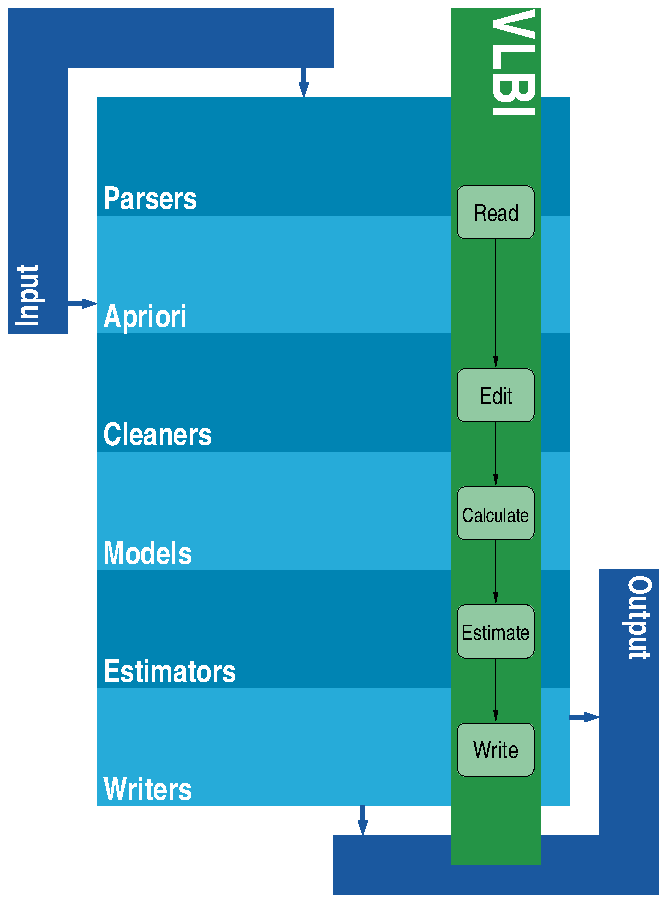
\includegraphics[width=0.8\linewidth]{kirkvik01}
\caption{\textbf{Where} architecture: The pipeline for the analysis of VLBI sessions.}
\label{fig:architecture}
\end{figure}

Figure~\ref{fig:architecture} shows the architecture and basic pipeline for a typical single session VLBI
analysis. In 2017 the theoretical VLBI delay model of the \textbf{Where} software was confirmed to be comparable with other
software packages~\cite{kirkvik2017b}.  This was done by utilizing the data and analysis from the VLBI Analysis Software
Comparison Campaign 2015~\cite{klopotek2016}.

\textbf{Where} uses a Kalman filter with a Modified Bryson-Frazier smoother (\cite{bierman2006}, \cite{gibbs2011}) for
estimation. Clocks and troposphere are modelled as continuous piecewise linear parameters. By default, the clocks and
the wet troposphere are estimated with one linear segment per hour, while the horizontal gradients use one linear segment per 6
hours. Normal equations as requested by the IVS are created following the method of~\cite{mysen2017}.

The \textbf{Where} software is available under an open source MIT license at \url{https://kartverket.github.io/where}.

\section{Verification and validation}

Lately, a lot of effort has been put into analyzing sessions from 1994 to 2016 to identify clock breaks and other issues
with the data. Furthermore, the estimator and writer components have been completed and a lot of testing has been done.
Several solutions have been submitted to the CCIVS for evaluation. Based on the feedback the
CCIVS several issues with the software has been resolved. Table \ref{tbl:solutions} summarizes the 
submitted solutions and their issues.

\begin{table*}[!htbp]
\caption{Solutions submitted to the CCIVS for testing. The first column indicates the solution number
and the second column shows which sessions that were analyzed. All 24 hour sessions for a given year were submitted.
The third column shows which parameters that were included in the submitted normal equations. The fourth and fifth
column describes the problems with the solutions and how these were improved in later solutions. }
\setlength{\extrarowheight}{5pt}
\setlength{\tabcolsep}{5pt}
\begin{tabularx}{\textwidth}{l|l|l|l|l}
\hline
\textbf{No.} & \textbf{Data} & \textbf{Parameters} & \textbf{Problems/Comments} & \textbf{Difference wrt to previous
solution} \\
\hline
1 & 2016 & \makecell[tl]{Station coordinates \\ EOP} & \makecell[tl]{Estimates too close to a priori \\ Low weight
factor in the combination} & \makecell[tl]{Initial solution} \\
\hline
2 & 1994--2016 & \makecell[tl]{Station coordinates \\ Source coordinates\\ EOP} & \makecell[tl]{Same as above
\\ Problems with source names} & \makecell[tl]{Software unchanged}\\
\hline
3 & 2013--2016 & \makecell[tl]{Station coordinates \\ EOP} & \makecell[tl]{Wrong sign on estimates \\ Worse weight
factor in combination \\ Offsets and high variability in EOP} & \makecell[tl]{Fixed bug that caused too small
estimates}
\\
\hline
4 & 2002--2016 & \makecell[tl]{Station coordinates \\ EOP} & \makecell[tl]{Variations in LOD \\ Otherwise OK} &
\makecell[tl]{Fixed bug with estimate sign \\ Updated EOP C04 file \\ Increased a priori standard deviations
for EOP} \\
\hline
5 & 2002--2016 & \makecell[tl]{Station coordinates \\ Source coordinates \\ EOP} & \makecell[tl]{Not analyzed yet} &
\makecell[tl]{Fixed bug with LOD sign \\ Corrected source names} \\
\hline
\end{tabularx}
\label{tbl:solutions}
\end{table*}

In March 2018 the first test solution was submitted to the CCIVS. It consisted of one year of
sessions (2016) and contained estimates for Earth Orientation Parameters (EOP) and station coordinates. Briefly after, a
solution with 23 years of processed sessions (1994-2016) was also submitted. The second solution also contained estimates for radio
source coordinates. These solutions were processed by the same setup and version of the software.

However, there were some problems with the submitted solutions. First of all, the radio source names were wrong for
those sources that are listed in the observation file with a different name than the official IERS name. This problem
has been resolved, but not yet verified by the CCIVS.

Secondly -- and more worrisome -- the estimates appeared to be extremely close to the a priori values. The first (and 
second) solution also contained large offsets in estimated station coordinates for some stations and the computed weight
 factor for the solution in the combination was too low.

The main problem was that when the Kalman filter iterated and removed outliers it did not estimate the parameters from
scratch, but rather estimated a correction to the previous estimate. It was this correction to the previous estimate 
that was wrongly used to generate the normal equations.

The implementation of the creation of the normal equations also contained some minor bugs. All these mistakes were
corrected in a new version of the software. A third solution with station coordinates and EOPs using sessions from 2013
to 2016 was then submitted at the end of May.

\begin{figure}[!htbp]
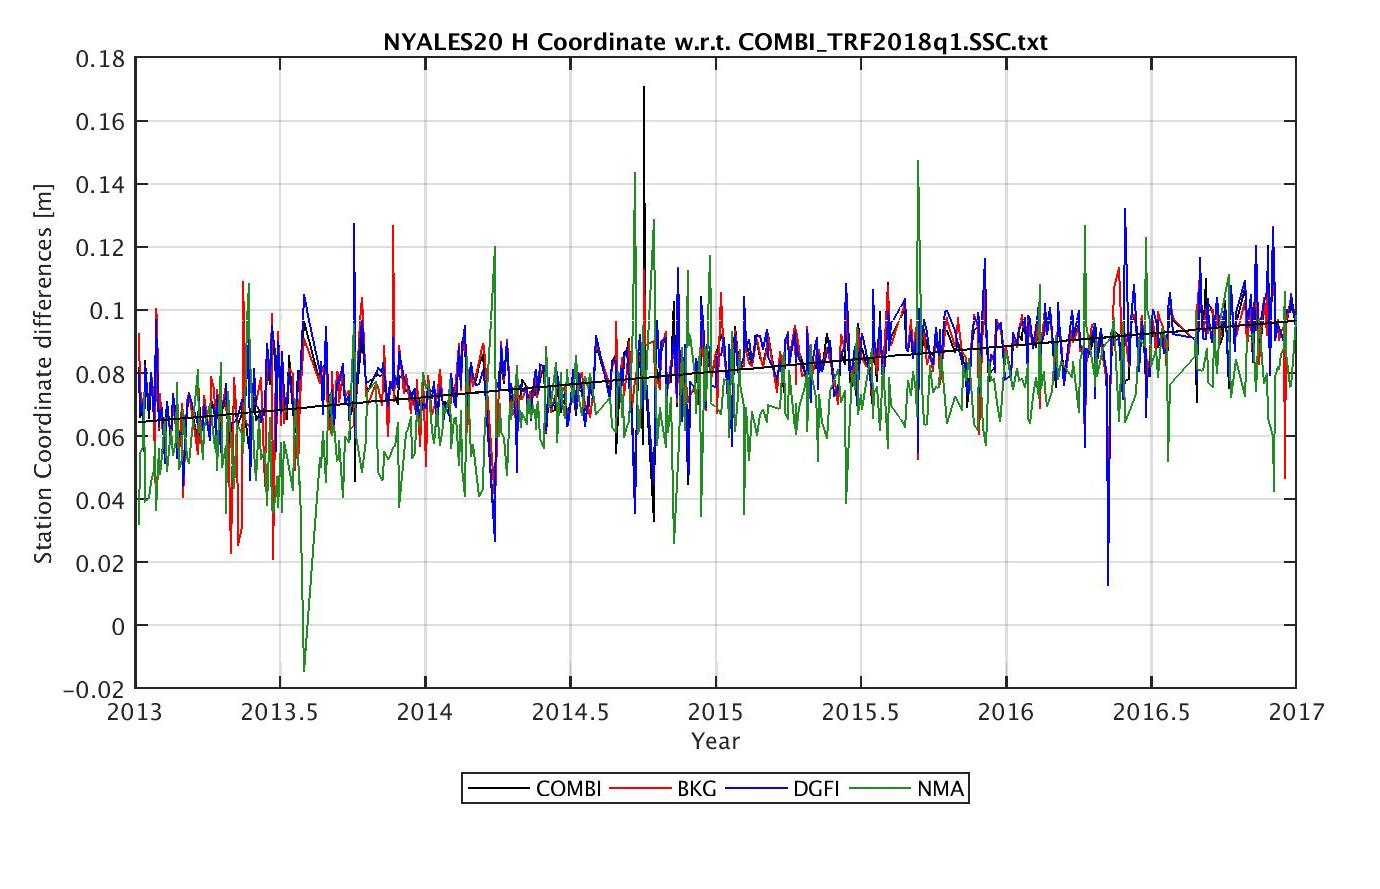
\includegraphics[width=\linewidth]{kirkvik02}
\caption{Difference between height component of NYALES20 and a reference frame solution from the third solution.
Provided by Sabine Bachmann, BKG.}
\label{fig:bad_nyal_h}
\end{figure} 

The magnitude of the estimates now seemed to be reasonable and the estimates were no longer too optimistic. But they
were still slightly different from the other analysis centers and the combined solution. They appeared to have the opposite
sign. This can be for instance be seen pretty clearly in the height component at Ny-{\AA}lesund in figure
\ref{fig:bad_nyal_h}.

In addition, the offsets observed in the previous solutions and the weight factor became worse instead of better. This
behaviour is also consistent with the sign error. The problem was traced back to the residual vector that
turned out to have the wrong sign.

There were also some problems with the EOPs. There was an offset in UT1-UTC and a large variability in the estimates for
most of the parameters compared to the other analysis centers.

The sign error was corrected and a updated version of the a priori EOP 14 C04 file was downloaded which had not been
updated locally since September 2017. Since then, IERS has made several changes and fixed problems with this time
series\footnote{http://hpiers.obspm.fr/iers/eop/eopc04/updateC04.txt}. The latest change in April 2018. Especially,
the UT1-UTC time series had large differences. The standard deviations for the EOP used in the a priori covariance matrix in the Kalman filter were also
increased, as some values were artifically low. The final values used are summarized in table \ref{tbl:sigmas}.

\begin{table}[!htbp]
\caption{Default a priori covariance matrix used in \textbf{Where}. The matrix is a diagonal matrix with $\sigma^2$ on the diagonal.}
%\setlength{\extrarowheight}{10pt}
\begin{tabularx}{\columnwidth}{X|r}
\hline
\textbf{Parameter} & $\sigma$ \\
\hline
\multicolumn{2}{l}{\textit{Constant parameters}} \\
\hline
Station coordinates      & 1\,m \\
UT1-UTC                  & 10\,ms \\
LOD                      & 10\,ms \\
Polar motion             & 100\,mas \\
Polar motion rate        & 100\,mas/d \\
Precession/Nutation      & 100\,mas \\
Radio source coordinates & $2.5\times 10^{-7}$\,rad \\
\hline
\multicolumn{2}{l}{\textit{Piecewise Linear Parameters (offset and rate)}} \\
\hline
Clock                   & 1\,m and 1\,m/h\\
Wet troposphere         & 1\,m and 1\,m/h \\
Horizontal gradients    & 1\,m and 1\,m/h \\
\hline
\end{tabularx}
\label{tbl:sigmas}
\end{table}

\begin{figure}[!htbp]
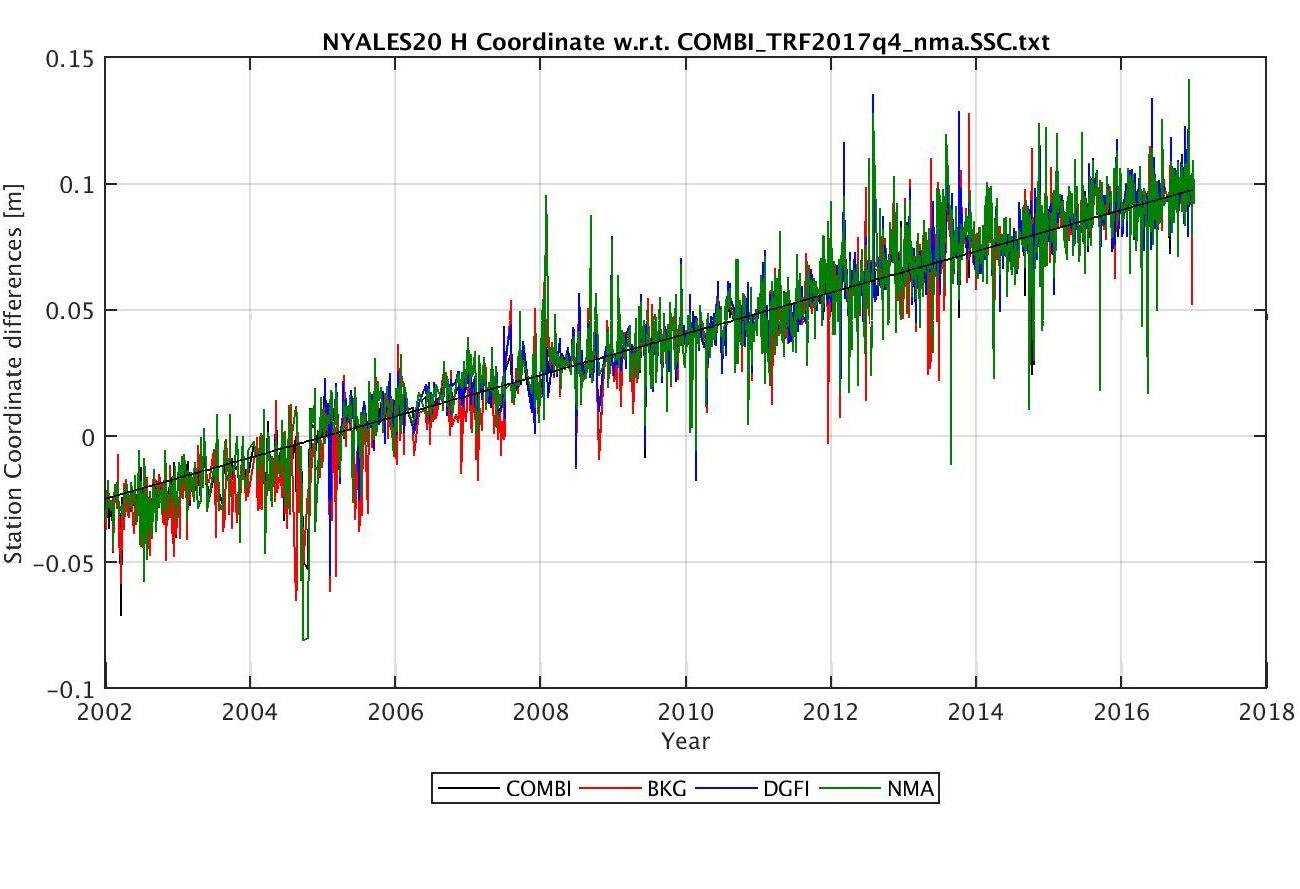
\includegraphics[width=\linewidth]{kirkvik03}
\caption{Difference between height component of NYALES20 and a reference frame solution from the fourth solution.
Provided by Sabine Bachmann, BKG.}
\label{fig:nyal_h}
\end{figure}

\begin{figure*}[!htbp]
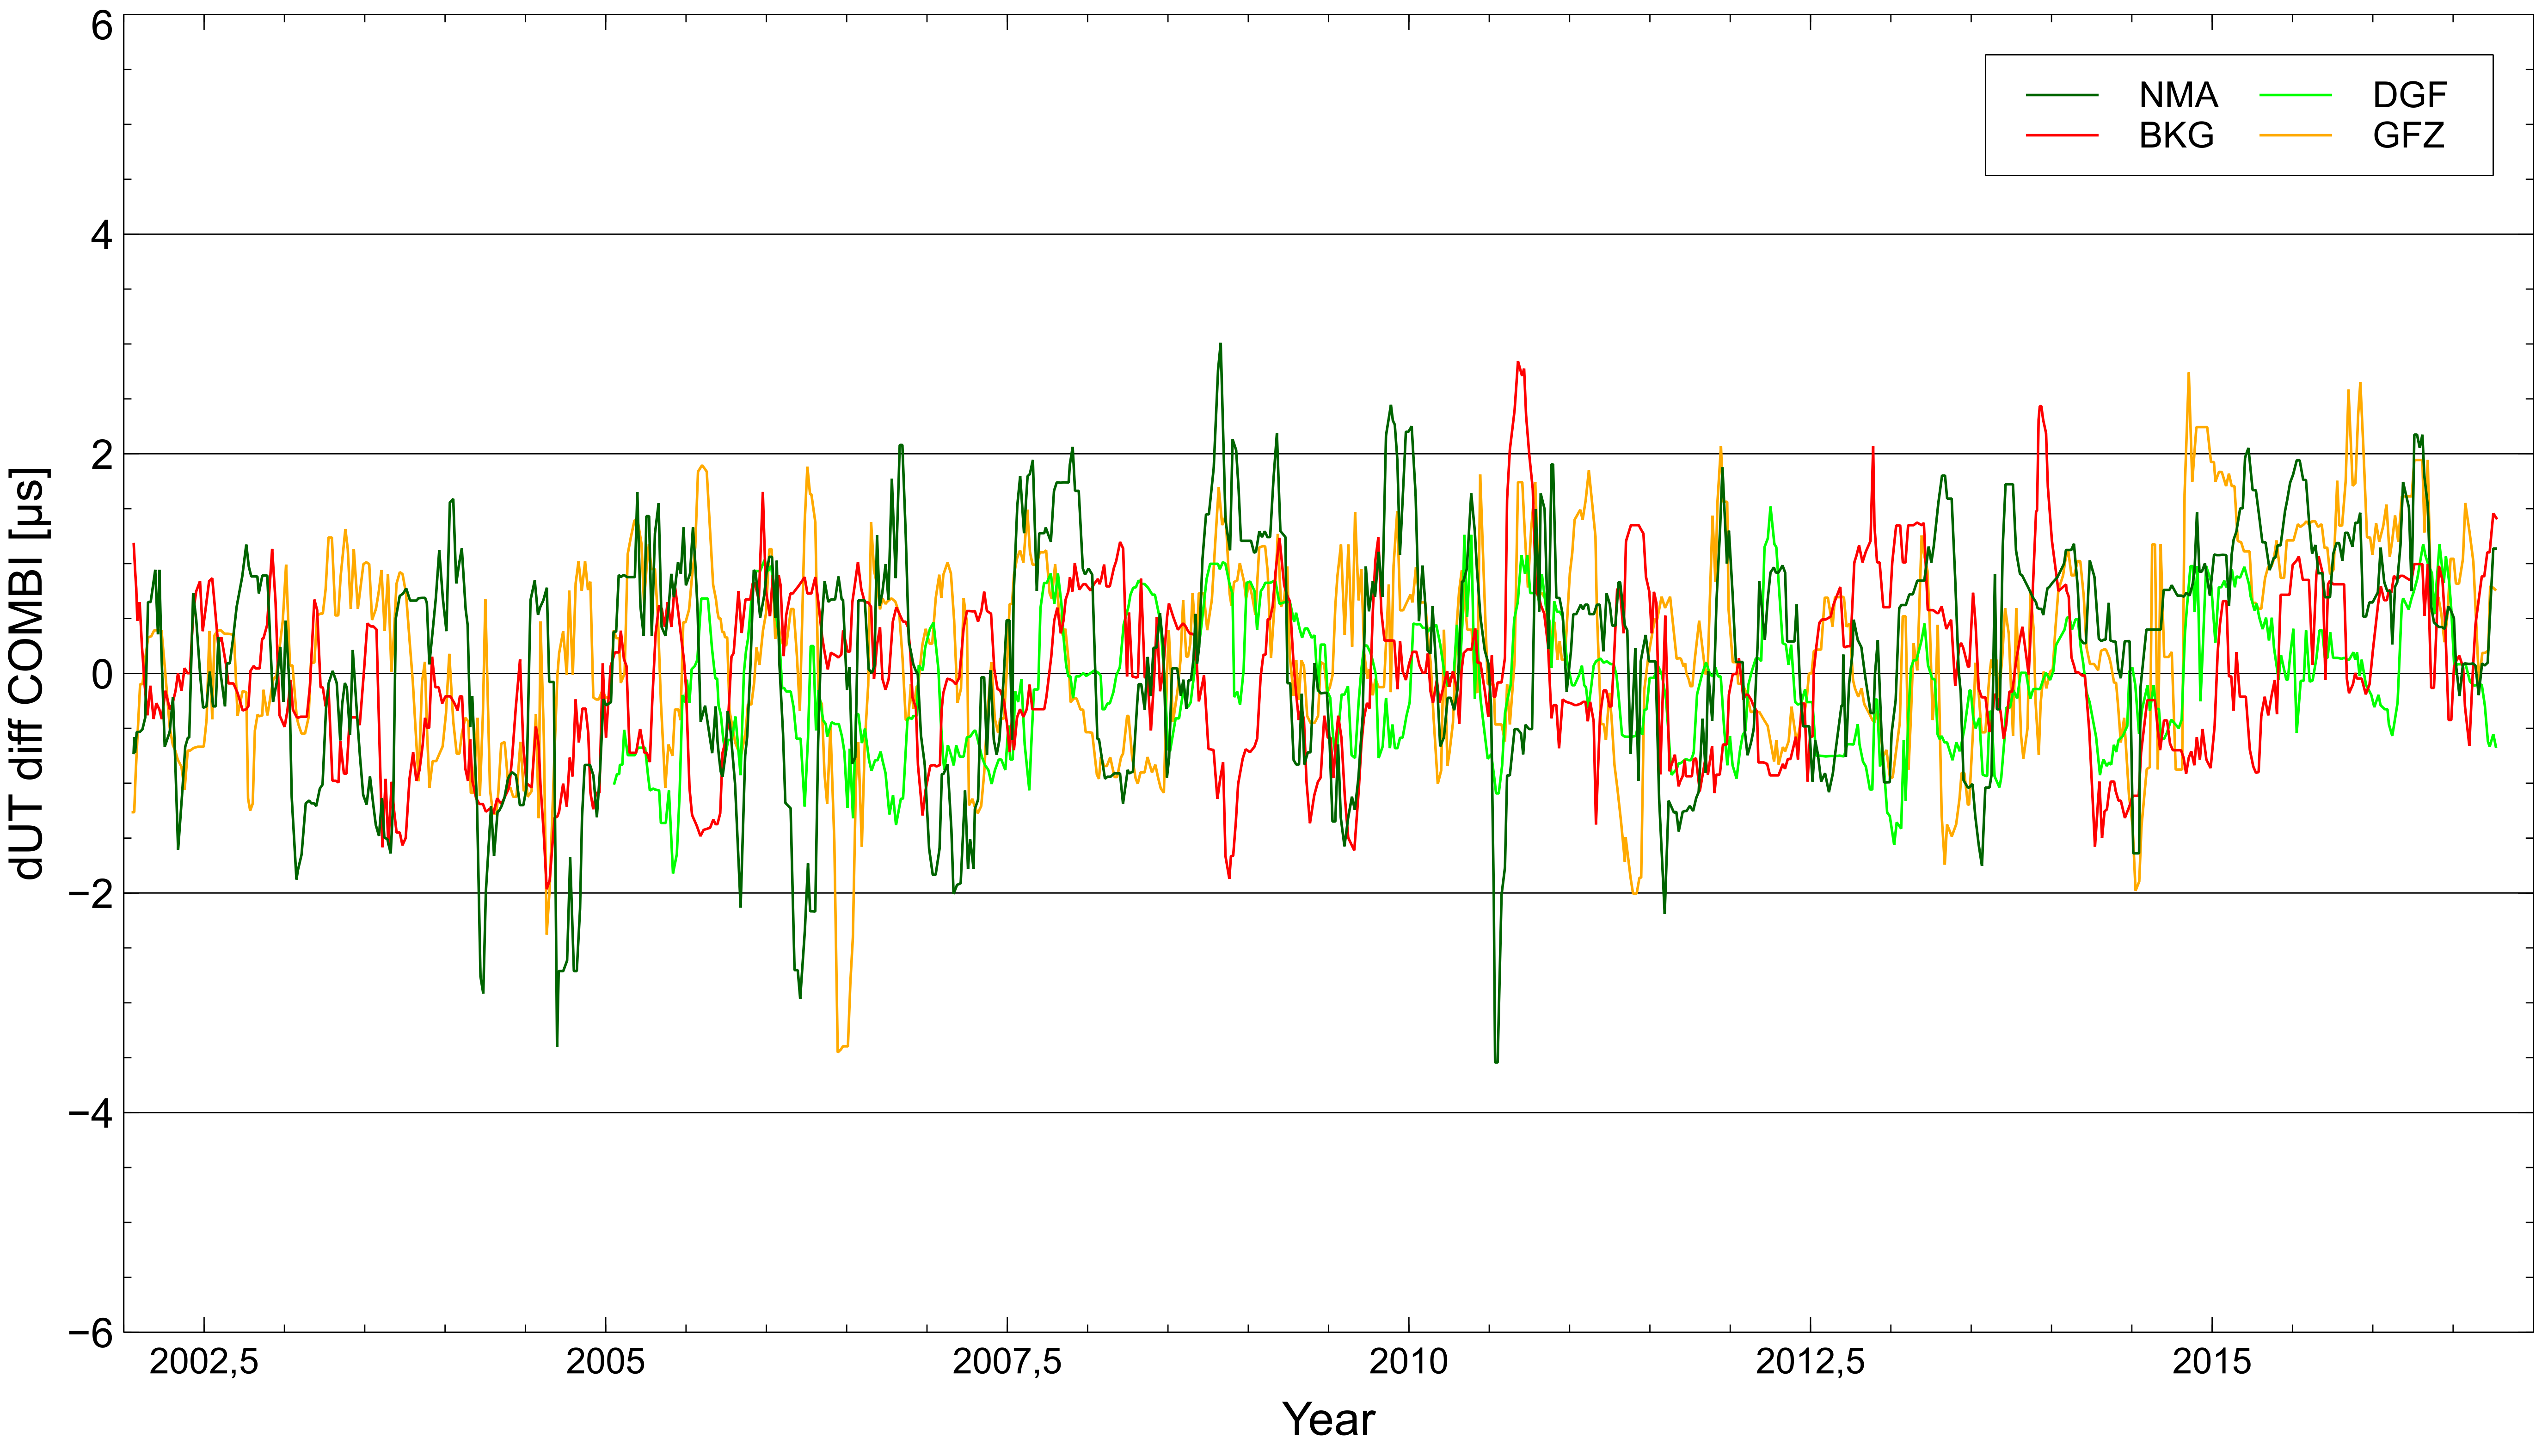
\includegraphics[width=\linewidth]{kirkvik04}
\caption{Difference between UT1-UTC and the combined solution for different analysis centers from the fourth solution.
Provided by Sabine Bachmann, BKG.}
\label{fig:dut}
\end{figure*}

\begin{figure*}[!htbp]
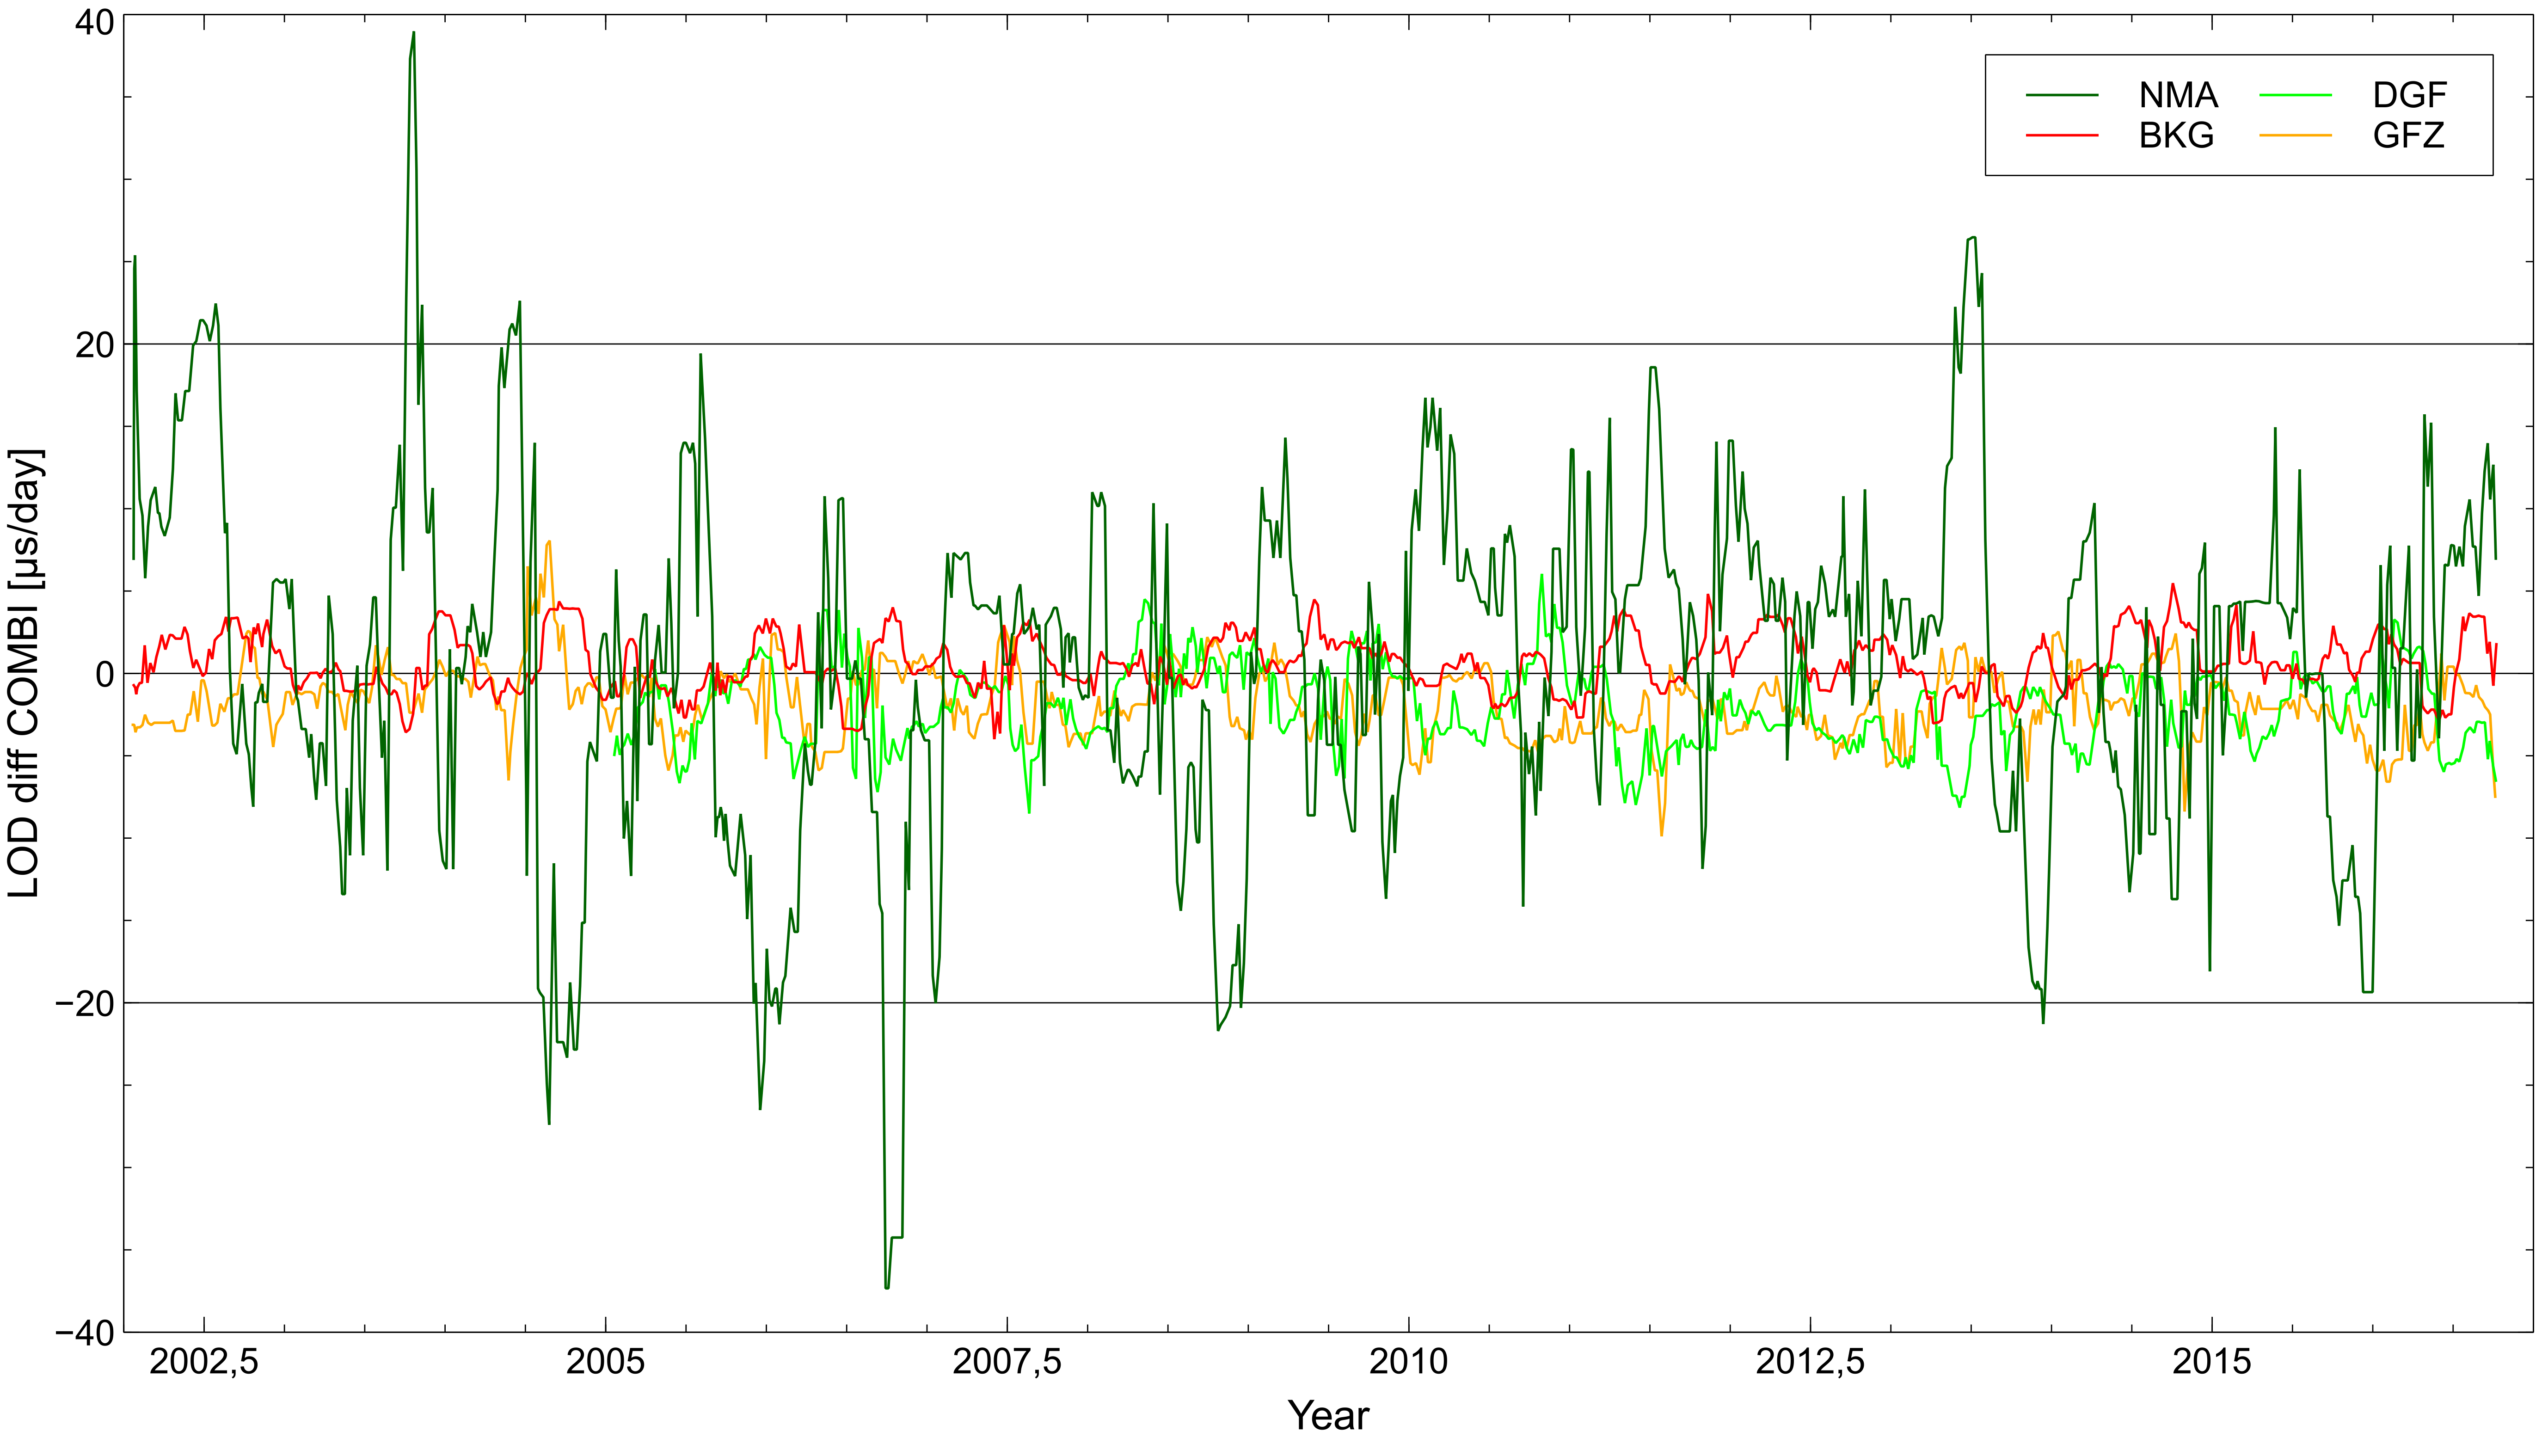
\includegraphics[width=\linewidth]{kirkvik05}
\caption{Difference between LOD and the combined solution for different analysis centers from the fourth solution.
Provided by Sabine Bachmann, BKG.}
\label{fig:lod}
\end{figure*}


A fourth solution was submitted with processed sessions from 2002--2016 at the end of June. This time the results were
more promising.
The station coodinates and EOP estimates seemed to be comparable with other analysis centers. For instance, figure
%\ref{fig:nyal_e}, \ref{fig:nyal_n} and
\ref{fig:nyal_h} shows the height component at NYALES20, which is clearly improved compared to figure
\ref{fig:bad_nyal_h}.
Figure \ref{fig:dut} shows the difference between estimated UT1-UTC and the combined solution. Figure \ref{fig:lod} shows the same but for LOD. The high variations in LOD is still a problem, but UT1-UTC and the
other EOPs (not shown here) agree well with other analysis centers.

A sign error in the partial derivatives of the LOD parameter was discovered and the sesssions from 2002 to 2016 were
processed again. This fifth, and currently final solution was submitted in August, but has not yet been analyzed by the
CCIVS. This LOD bugfix is expected to improve the LOD estimates, but it is still an open question on
how to compute a good a priori value for LOD, so a bit more work might be needed. In addition, this solution
reintroduced radio source coordinates, but with correct source names. Feedback on the fifth
solution is anticipated soon.


% \begin{figure}[!htbp]
% 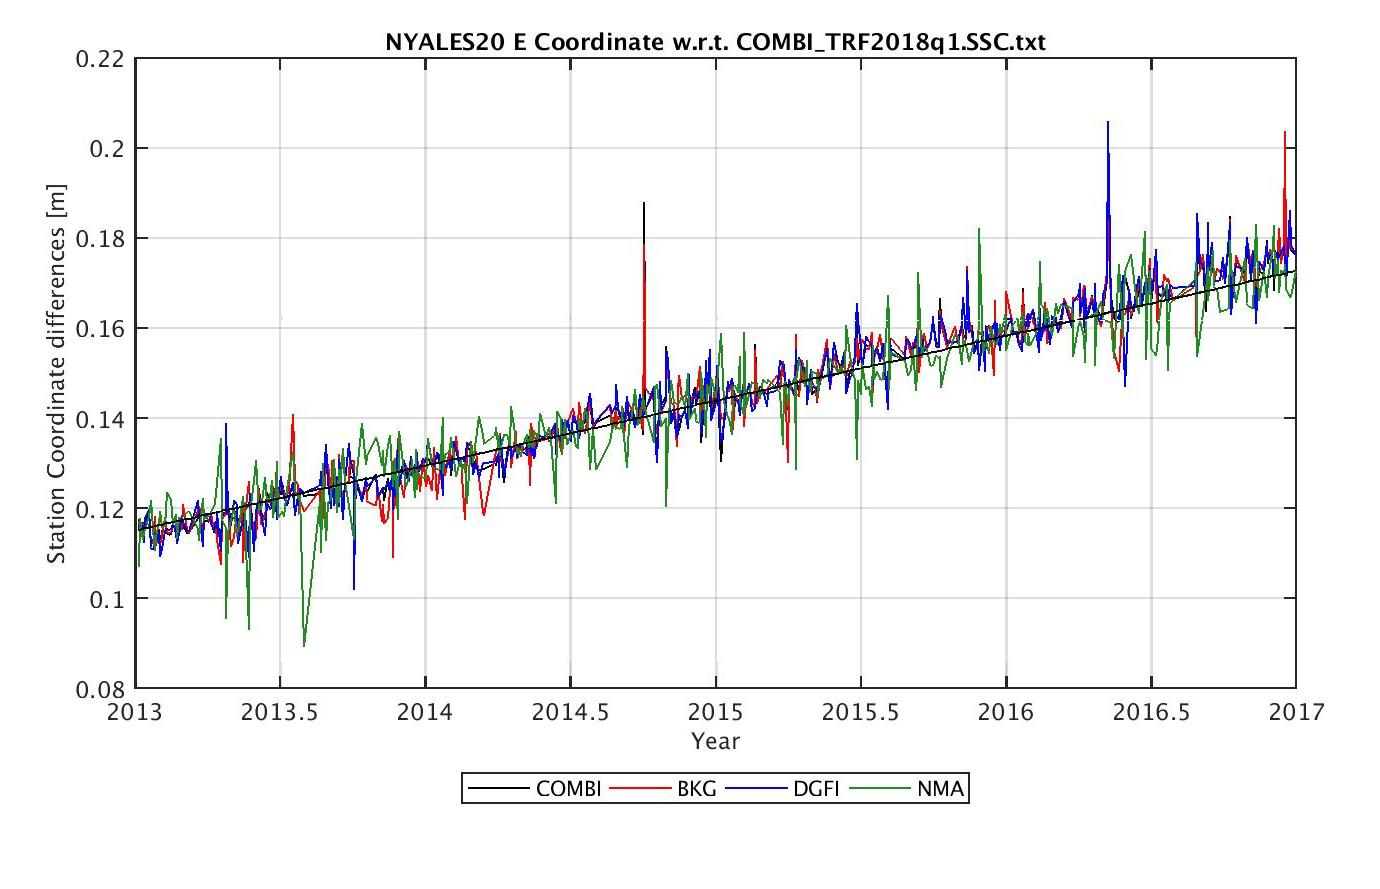
\includegraphics[width=\linewidth]{NYALES20-E_diff-trf}
% \caption{Difference between east component of NYALES20 and a reference frame solution. Provided by Sabine Bachmann,
% BKG.}
% \label{fig:nyal_e}
% \end{figure} 
% 
% \begin{figure}[!htbp]
% 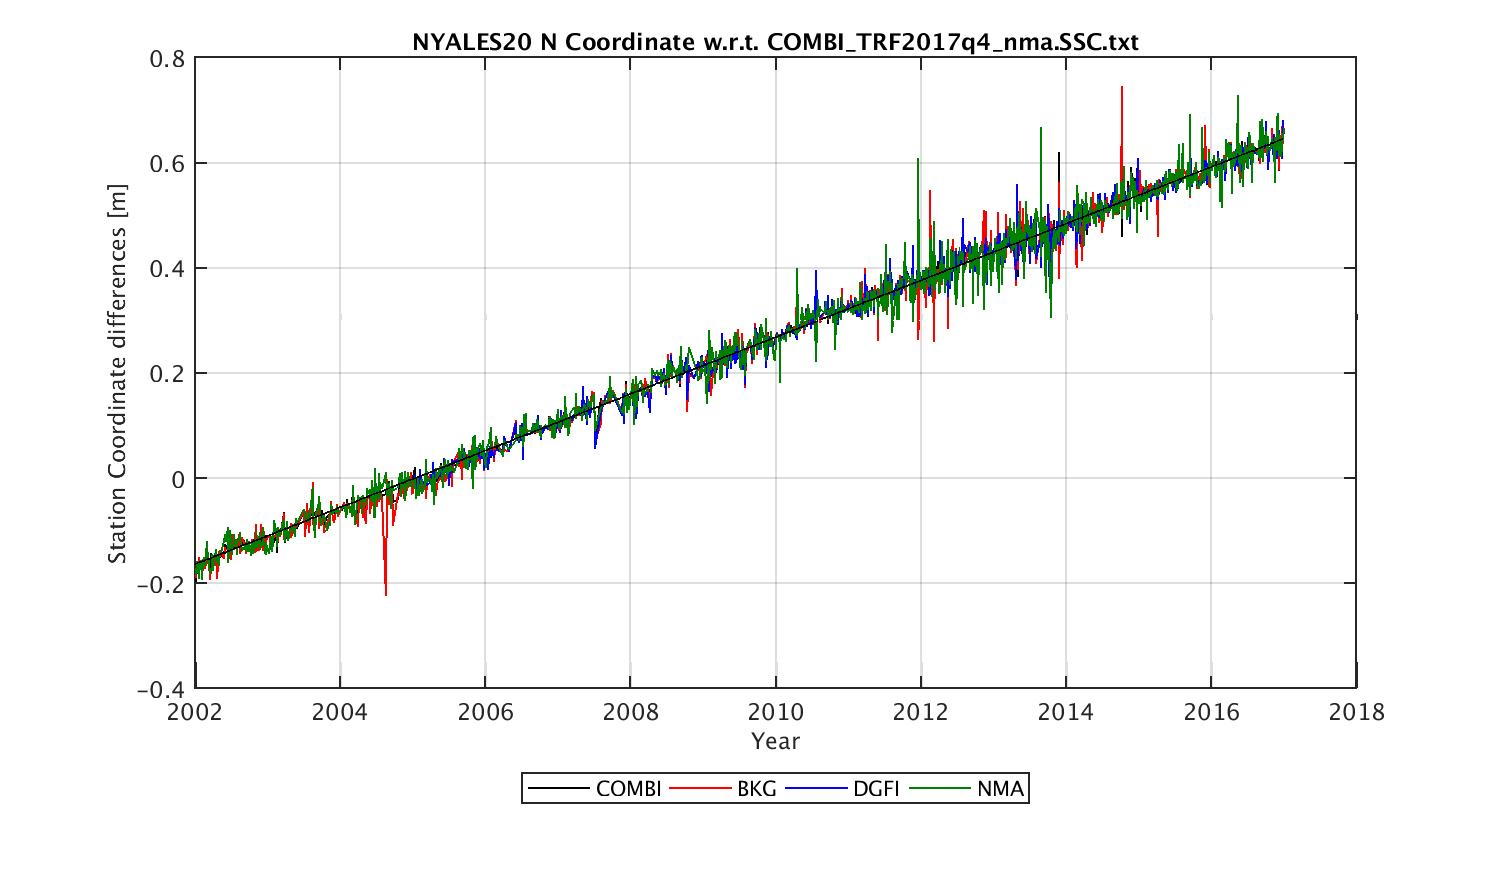
\includegraphics[width=\linewidth]{NYALES20-N_diff-trf}
% \caption{Difference between north component of NYALES20 and a reference frame solution. Provided by Sabine Bachmann,
% BKG.}
% \label{fig:nyal_n}
% \end{figure} 
 

\section{Future work}

The immediate plan is to continue to submit analyzed sessions to the CCIVS to improve the quality of
the solution. When the estimates of station coordinates and the EOP seem reasonable, the source coordinates will be
added again. Also, with the disappearance of the NGS card file format the vgosDb file format parser needs to be tested
more extensively and improved.

When the quality is approved, the next step is to start analyzing regularly the R1 and R4 sessions and to establish good
routines for upholding the timeliness requirement. The plan is to start regular analysis by the end of 2018. This step
will involve a different set of challenges such as automation of the analysis and having qualified personnel available
during vacations.

In addition, outliers should be studied more closely. Some sessions do not have enough usable observations to estimate
the full set of parameters. These sessions require special handling and complicates the road to automating the analysis
as much as possible.

Finally, models needs to be updated as new conventions and analysis strategies are being implemented in preparation for
the next international terrestrial reference frame solution projected for 2020. 

%\section{Future work}



%  Code to include a single column figure through \includegraphics.
% \begin{figure} and \end{figure} make this single column.
% If the figure is too wide, it will overwrite text in the other column.
% Figures and their captions should be left-justified.
% So please do not add commands to center them.
% The class file will automatically perform the left-justification.
%  \begin{figure}[htb!]  Please specify the file extension as part of the figure file name. The formats of jpg, png and
% pdf can be used.
% If you have only one paper, the files should be named papername##.extension, where papername is the name of the paper
% (from papername.tex) and ## is the number of each successive file name (e.g., lebail01.jpg, lebail02.png, ...,
% lebail10.jpg, etc.) If you have two or more papers, the files should be named papernameN##.extension, where N is the
% number of the paper (e.g., gipson101.jpg and gipson102.png for paper 1, gipson201.pdf for paper 2, gipson301.png for
% paper 3 and so on).
%  \includegraphics[width=.5\textwidth]{ivs-gm-template01.jpg} %%%%  The caption should not be preceded by Figure 1.
% %%%%  Please just enter your desired caption, such as:
% %%%%         Equipment at our station.
% \caption{Example of figure from .jpg file.} \label{first-unique-label} \end{figure}


% \begin{figure}
%     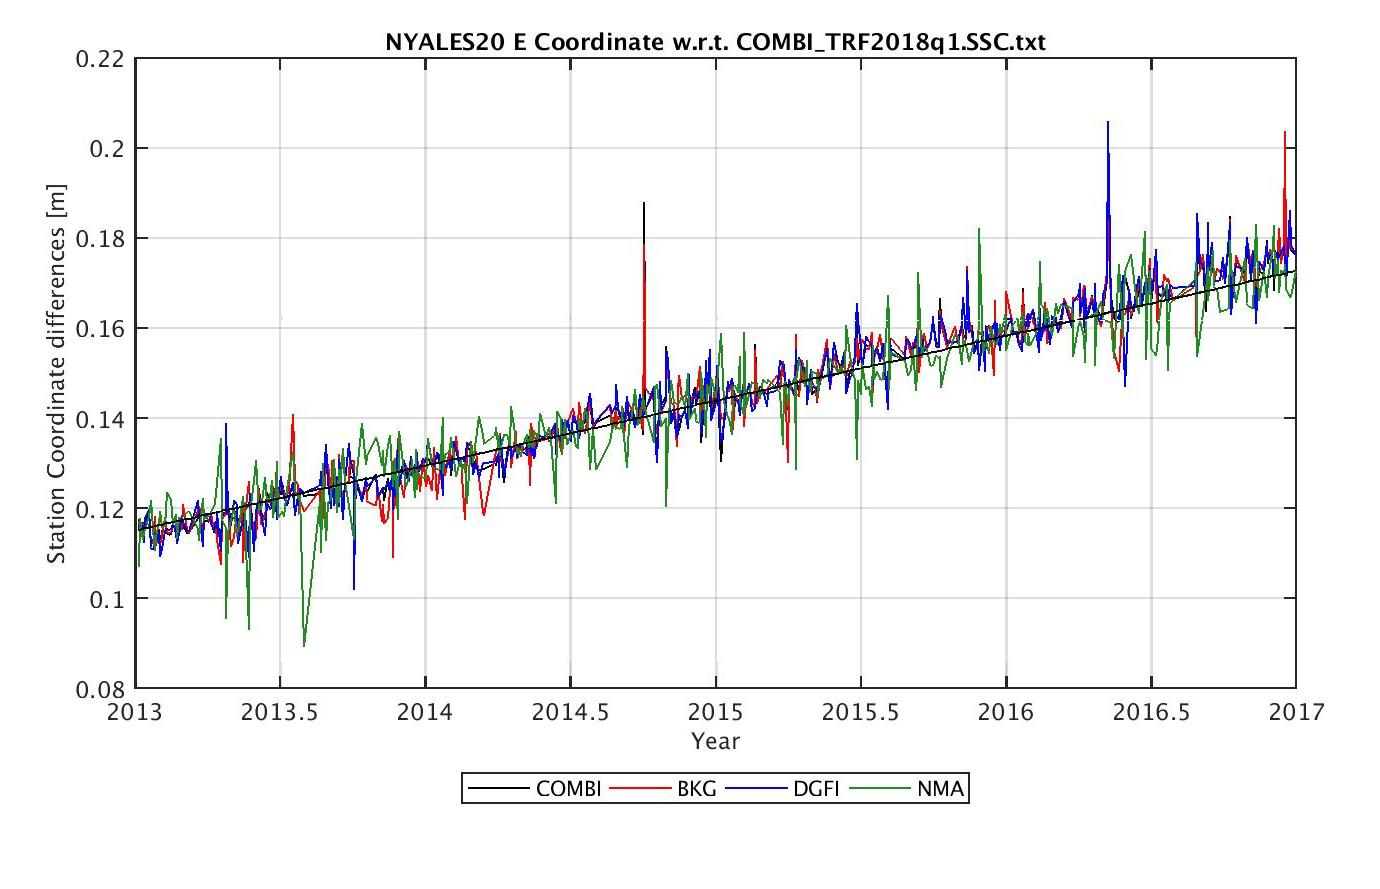
\includegraphics[width=\linewidth]{NYALES20-E_diff-trf}
%     \caption{East}
%     \label{fig:nyal_e}
% \end{figure}
%
% \begin{figure}
%     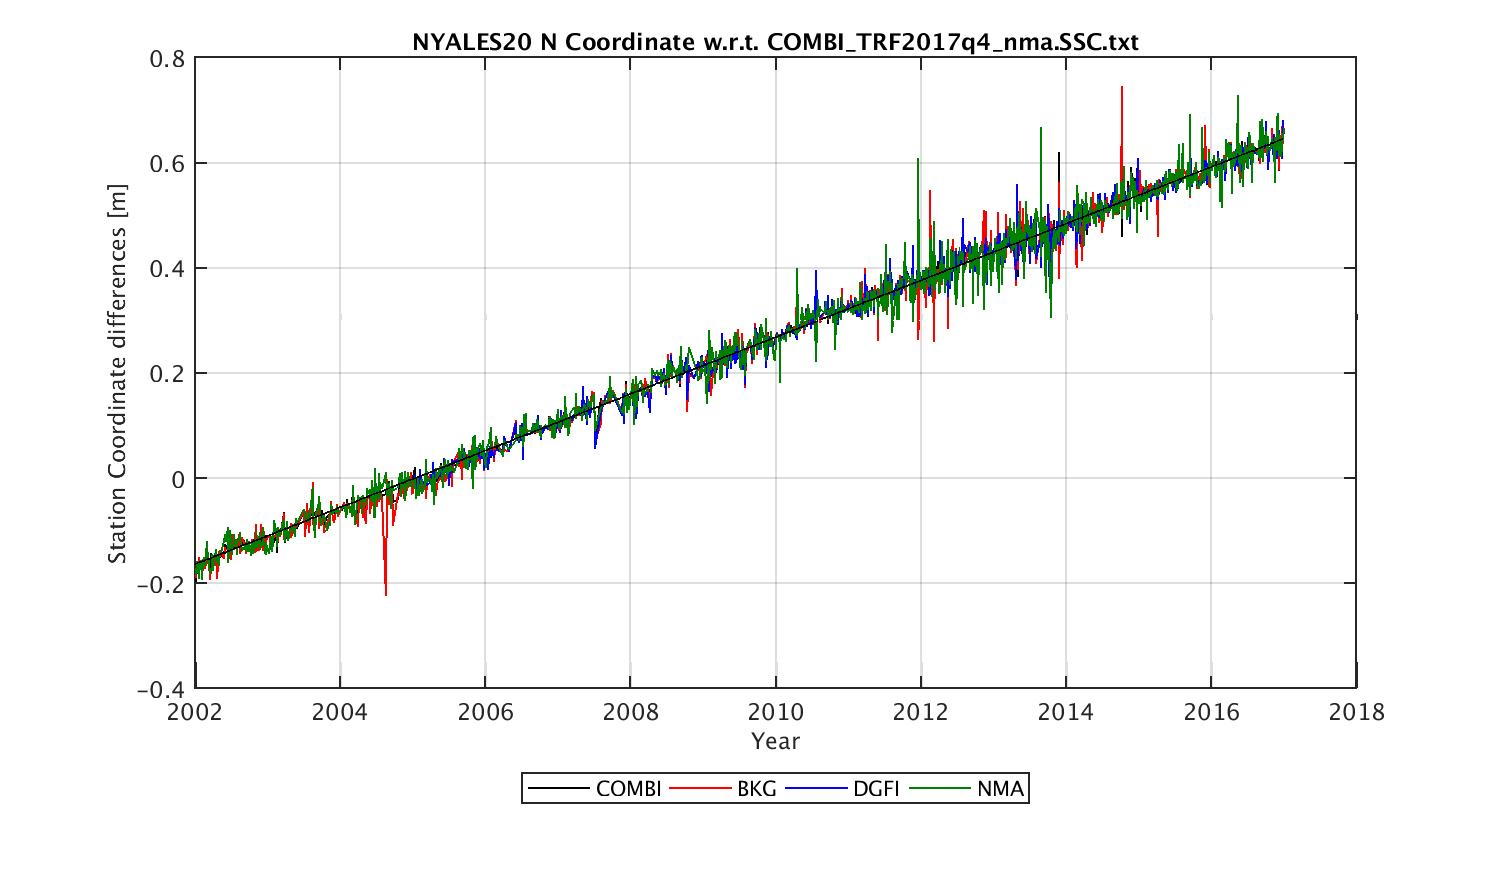
\includegraphics[width=\linewidth]{NYALES20-N_diff-trf}
%     \caption{North}
%     \label{fig:nyal_n}
% \end{figure}



%
% Code to use \includegraphics to include a figure that spans two columns.
% \begin{figure*} and \end{figure*} will allow the figure to Span
% two columns.  If the figure is too narrow, it will leave blank space
% in the other column.
% Figures and their captions should be left-justified.
% So please do not add commands to center them.
% The class file will automatically perform the left-justification.
%
%\begin{figure*}[htb!]
% Please see the above figure example for naming conventions for the
% figure file.
%\includegraphics[width=16.0cm]{ivs-gm-template02.png}
% Please do not precede the caption by Figure 2.
% Please just enter your desired text.
%\caption{Example of figure from .png file.}
%\label{second-unique-label}
%\end{figure*}
%
% Code to include a single column table.
% Other table formats may be used also.
% Tables and their captions should be left-justified.
% So please do not add commands to center them.
% The class file will automatically perform the left-justification.
%
% \begin{table}[htb!]
% \caption{Caption for Table 1.}
% \begin{tabular}{|l|c|c|r|} \hline
% Heading 1 & Heading 2 & Heading 3 & Heading 4\\
% \hline
% Value a1 & Value a2 & Value a3 &          \\
% Value b1 &          & Value b3 & Value b4 \\
% Value c1 & Value c2 & Value c3 &          \\
% Value d1 & Value d2 & Value d3 & Value d4 \\
% Value e1 & Value e2 & Value e3 & Value e4 \\
% \hline
% \end{tabular}
% \label{third-unique-label}
% \end{table}




%
% Code to include a two column table.
% Other table formats may be used also.
% Tables and their captions should be left-justified.
% So please do not add commands to center them.
% The class file will automatically perform the left-justification.
%
% \begin{table*}[htb!]
% \caption{Caption for Table 2.}
% \begin{tabular}{|l|c|c|r|l|c|c|r|} \hline
% Heading 1 & Heading 2 & Heading 3 & Heading 4 & Heading 5 & Heading 6 & Heading 7 & Heading 8\\
% \hline
% Value a1 & Value a2 & Value a3 &          & Value a5 & Value a6 & Value a7 & Value a8 \\
% Value b1 &          & Value b3 & Value b4 &          &          & Value b7 & Value b8 \\
% Value c1 & Value c2 & Value c3 &          & Value c5 & Value c6 & Value c7 &          \\
% Value d1 & Value d2 & Value d3 & Value d4 & Value d5 & Value d6 &          &          \\
% Value e1 & Value e2 & Value e3 & Value e4 & Value e5 &          & Value e7 &          \\
% Value f1 & Value f2 & Value f3 & Value f4 & Value f5 &          & Value f7 &          \\
% Value g1 &          & Value g3 & Value g4 & Value g5 & Value g6 & Value g7 & Value g8 \\
% \hline
% Value h1 & Value h2 & Value h3 &          & Value h5 & Value h6 & Value h7 & Value h8 \\
% Value i1 &          & Value i3 & Value i4 &          &          & Value i7 & Value i8 \\
% Value j1 & Value j2 & Value j3 &          & Value j5 & Value j6 & Value j7 &          \\
% Value k1 & Value k2 & Value k3 & Value k4 & Value k5 & Value k6 &          &          \\
% Value l1 & Value l2 & Value l3 & Value l4 & Value l5 &          & Value l7 &          \\
% Value m1 & Value m2 & Value m3 & Value m4 & Value m5 &          & Value m7 &          \\
% Value n1 &          & Value n3 & Value n4 & Value n5 & Value n6 & Value n7 & Value n8 \\
% \hline
% Value o1 & Value o2 & Value o3 &          & Value o5 & Value o6 & Value o7 & Value o8 \\
% Value p1 &          & Value p3 & Value p4 &          &          & Value p7 & Value p8 \\
% Value q1 & Value q2 & Value q3 &          & Value q5 & Value q6 & Value q7 &          \\
% Value r1 & Value r2 & Value r3 & Value r4 & Value r5 & Value r6 &          &          \\
% Value s1 & Value s2 & Value s3 & Value s4 & Value s5 &          & Value s7 &          \\
% Value t1 & Value t2 & Value t3 & Value t4 & Value t5 &          & Value t7 &          \\
% Value u1 &          & Value u3 & Value u4 & Value u5 & Value u6 & Value u7 & Value u8 \\
% \hline
% Value v1 & Value v2 & Value v3 &          & Value v5 & Value v6 & Value v7 & Value v8 \\
% Value w1 &          & Value w3 & Value w4 &          &          & Value w7 & Value w8 \\
% Value x1 & Value x2 & Value x3 &          & Value x5 & Value x6 & Value x7 &          \\
% Value y1 & Value y2 & Value y3 & Value y4 & Value y5 & Value y6 &          &          \\
% Value z1 & Value z2 & Value z3 & Value z4 & Value z5 &          & Value z7 &          \\
% \hline
% \end{tabular}
% \label{fourth-unique-label}
% \end{table*}
%
% Please see the first two figures for detailed information
% about using figures.
%
% \begin{figure*}[htb!]
% \includegraphics[width=16.0cm]{ivs-gm-template03.pdf}
% \caption{Example of figure from .pdf file.}
% \label{fifth-unique-label}
% \end{figure*}
%
% The acknowledgements section is optional.  If used, the section line should
% be:
%      \section*{Acknowledgements}

\section*{Acknowledgements}

Thanks to Sabine Bachmann (BKG) at the IVS Combination Center for analyzing our solutions and providing
great feedback and insights.
%
% The bibliography section is optional.
%
% Here is a section with some examples.
% But the entries are free-format --- essentially,
%  \bibitem{unique-label}
%  text
%
%%%%%\begin{thebibliography}{99}
%%%%%\bibitem{Abbondanza2012}
%%%%%C.~Abbondanza and P.~Sarti.
%%%%%Impact of network geometry, observation schemes and telescope structure deformations on local ties:
%%%%%simulations applied to Sardinia Radio Telescope.
%%%%%\emph{Journal of Geodesy}, 86(3), doi:10.1007/s00190-011-0507-6, 181--192, 2012.
%%
%%%%%\bibitem{Artz}
%%%%%Thomas Artz, Judith Leek, Axel Nothnagel, and Maike Schumacher.
%%%%%VLBI Intensive Sessions Revisited.
%%%%%In D.~Behrend and K.~Baver, editors, \emph{International
%%%%%  VLBI Service for Geodesy and Astrometry 2012 General Meeting Proceedings},
%%%%%  NASA/CP-2012-217504, pages 276--280, 2012.
%%%%%%%
%%%%%\bibitem{VieVS}
%%%%%Matthias Madzak, Sigrid B\"ohm, Hana Kr\'asn\'a, and Lucia Plank.
%%%%%Vienna VLBI Software Version 2.1 User Manual
%%%%%Web document http://vievs.geo.tuwien.ac.at/fileadmin/editors/VieVS/documents/vievsDoc.pdf
%%%%%%
%%%%%\end{thebibliography}
%
\begin{thebibliography}{99}
\providecommand{\url}[1]{\texttt{#1}}
\providecommand{\urlprefix}{URL }
\expandafter\ifx\csname urlstyle\endcsname\relax
\providecommand{\doi}[1]{doi:\discretionary{}{}{}#1}\else
\providecommand{\doi}{doi:\discretionary{}{}{}\begingroup
\urlstyle{rm}\Url}\fi

\Urlmuskip=0mu plus 1mu\relax

\bibitem{behrend2013}
Behrend, D., {Data Handling within the International {VLBI} Service},
\emph{Data Science Journal}, 12, pp. WDS81--WDS84, 2013,
\doi{10.2481/dsj.WDS-011}.

\bibitem{bierman2006}
Bierman, G., \emph{Factorization Methods for Discrete Sequential Estimation},
Dover Books on Mathematics Series, Dover Publications, 2006.

\bibitem{gibbs2011}
Gibbs, R.~G., Square root modified bryson-frazier smoother, \emph{IEEE
Transactions on Automatic Control}, 56(2), pp. 452--456, 2011,
\doi{10.1109/TAC.2010.2089753}.

\bibitem{kierulf2010}
Kierulf, H.~P., et~al., {VLBI} analysis with the multi-technique software
{GEOSAT}, in Behrend, D., Baver, K.~D. (eds.), \emph{VLBI2010: From Vision to
Reality}, vol. NASA/CP-2010-215864 of \emph{IVS General Meeting Proceedings},
pp. 207--211, IVS, 2010.
%\newline\urlprefix\url{ivscc.gsfc.nasa.gov/publications/gm2010/kierulf.pdf}

\bibitem{kirkvik2017a}
Kirkvik, A.-S., Norwegian mapping authority analysis center {IVS} biennial
report 2015--2016, in Baver, K.~D., Behrend, D., Armstrong, K.~L. (eds.),
\emph{International VLBI Service for Geodesy and Astrometry 2015+2016
Biennial Report}, 2017.

\bibitem{kirkvik2017b}
Kirkvik, A.-S., et~al., Where - a new software for geodetic analysis, in Haas,
R., Elgered, G. (eds.), \emph{Proceedings of the 23rd European VLBI Group for
Geodesy and Astrometry Working Meeting}, 2017.

\bibitem{klopotek2016}
Klopotek, G., et~al., Results from the {VLBI} analysis software comparison
campaign 2015, in Behrend, D., Baver, K.~D., Armstrong, K.~L. (eds.),
\emph{New Horizons with VGOS}, vol. NASA/CP-2016-219016 of \emph{IVS General
Meeting Proceedings}, pp. 203--207, IVS, 2016.
%\newline\urlprefix\url{ftp://ivscc.gsfc.nasa.gov/pub/general-meeting/2016/pdf/042\_klopotek\_etal.pdf}

\bibitem{mysen2017}
Mysen, E., On the equivalence of {K}alman filtering and least-squares
estimation, \emph{Journal of Geodesy}, 91(1), pp. 41--52, 2017,
\doi{10.1007/s00190-016-0936-3}.

\bibitem{schuh2012}
Schuh, H., Behrend, D., {VLBI}: A fascinating technique for geodesy and
astrometry, \emph{Journal of Geodynamics}, 61, pp. 68 -- 80, 2012,
\doi{https://doi.org/10.1016/j.jog.2012.07.007}.
%\newline\urlprefix\url{http://www.sciencedirect.com/science/article/pii/S0264370712001159}

\end{thebibliography}

\end{document}
